\chapter{Tutorials}

\textbf{Preliminaries}\\
Before diving into the tutorials, here are some preliminaries that will help you guide easily through them.

\begin{itemize}
    \item A PSD simulation is performed in three steps: preprocessing, solving, and postprocessing. 
    \item Domain: denoted by $\Omega$ is a a $n$-dimensional solid body such that $\Omega \subset \mathbbm{R}^n$ with $n=2$   for 2D problems or  $n=3$ for 3D problems.
    \item Finite element mesh: denoted by $\Omega^h$ with mesh size $h$. Mesh can be triangular in 2D and tetrahedral in 3D.
    \item MPI processes for simulation: denoted by $\np$ these are the total MPI ranks that will work in parallel to solve the problem.
    \item Partitioned mesh: denoted by $\{ \Omega ^h_i \}_{i=1}^{\np}$ these are set of subdomains which are held by each MPI rank during a parallel simulation.
\end{itemize}

\section{Linear Elasticity}
Linear Elasticity is a mathematical approximation of solid object deformation caused by prescribed loading conditions. It is a simplification of the more general nonlinear theory of elasticity. PSD allows for solving Linear Elasticity problems both in sequential and in parallel. We shall discuss how to do so in details within this section.


PSD is a FEM based solver, to solve a given physics it heavily relies on the variational formulations of the underlying physics. Let us begin with writing the variational formulation of system of  Elasticity in which the primary unknown is the displacements vector $\bu=\{u_j\}^n_{j=1}$. In the Lagrangian FE framework for searching the unknown nodal displacements vector $\bu^h=\{u^h_j\}^n_{j=1}$ the variational formulation of system of  Elasticity reads,
%
%
\begin{equation}\label{Eq:Varf}
\forall i \in \llbracket 1; N_{\text p} \rrbracket,  \int_{\Omega^h_i}\sig(\buh) : \eps(\bvh) = \int_{\partial\Omega^h_{i,\text{N}}} \mathbf{f}\cdot\bvh \, \quad\forall\,\bvh\in\mathbb{V}^h,\buh\in\mathbb{V}^h,
\end{equation}
%
here,  $\buh$ is in fact the FE trial function and $\bvh=\{v^h_j\}^n_{j=1}$ is the FE test function.

\begin{equation}\label{Eq:LinearElasticity}
\forall i \in \llbracket 1; N_{\text p} \rrbracket, 
\int_{\Omega^h_i}\lambda\nabla\cdot\buh\nabla\cdot\bvh + \int_{\Omega^h_i}2\mu\boldsymbol\varepsilon(\buh):\boldsymbol\varepsilon(\bvh)-\int_{\Omega^h_i}\mathbf{f}\cdot\bvh=0, \quad\forall\bvh\in[H^1_0(\Omega^h_i)]^n 
\end{equation}

In these formulations $\lambda$ and $\mu$ are the Lame's parameters, $\mathbf{f}$ is the body force vector.  

\subsection{PSD simulation of 2D bar problem bending under own body weight \label{sec:2d-bar-load}}

To showcase the usage of Linear elasticity, we shall discuss here an example of a 2D bar, which bends under its own load. The bar ---$5\times1$~\si{\square\meter} in area-- is made up of material with $\rho=8\text e3$, $E=200\text e9$, and $\nu=0.3$.

\begin{figure}[htbp]
    \centering
    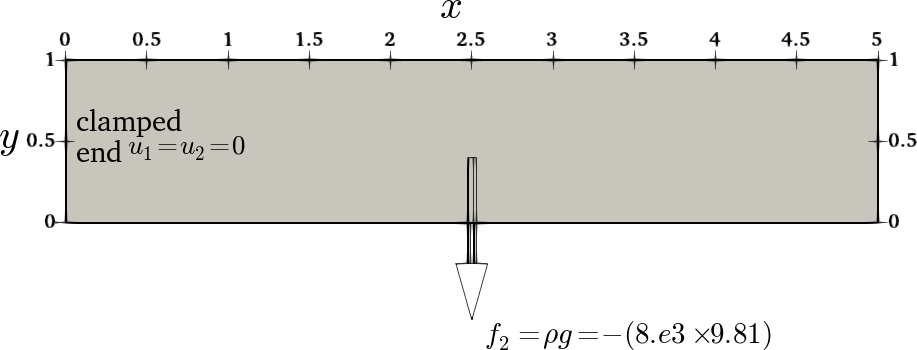
\includegraphics[align=t,width=.44\textwidth]{./Images/2d-bar.png}\hspace{.1\textwidth}
    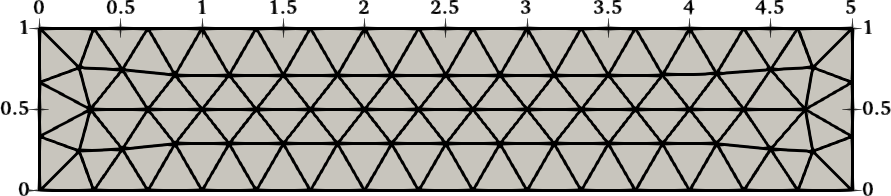
\includegraphics[align=t,width=.44\textwidth]{./Images/2d-bar-mesh.png}
    \caption{2D bar clamped at left end and bending under own load. Geometry (left) and mesh (right).}
    \label{fig:2Dbar}
\end{figure} 

\textbf{Step 1: Preprocessing}

First step in a PSD simulation is ``PSD preprocessing'', at this step you tell PSD what kind of physics, boundary conditions, approximations, mesh, etc are you expecting to solve.
For ``PSD Preprocessing'' go to any folder, launch \lstinline[style=Linux]!PSD_PreProcess! from the terminal with the following command:
\begin{lstlisting}[style=BashInputStyle]  
PSD_PreProcess -problem linear-elasticity -dimension 2 -bodyforceconditions 1 -dirichletconditions 1 -postprocess u
\end{lstlisting}
%
After the ``PSD Preprocessing'' runs successfully you should see many files with \lstinline[style=Linux]!.edp! extension in your folder. \textit{What do the arguments mean ?}   \lstinline[style=Linux]! -problem linear-elasticity! means that we will be solving linear-elasticity problem, \lstinline[style=Linux]! -dimension 2! means it is a 2D simulation, \lstinline[style=Linux]!-bodyforceconditions 1! with body force; \lstinline[style=Linux]!-dirichletconditions 1! says we have one Dirichlet border; and \lstinline[style=Linux]! -postprocess u! means we would like to have ParaView post processing files. The input properties ``$E,\nu$'' can be mentioned in \lstinline[style=Linux]! ControlParameters.edp!, change \lstinline[style=Linux]! E  = 200.e9!, and \lstinline[style=Linux]! nu = 0.3;!. The volumetric body force condition is mentioned in the same file via variable \lstinline[style=Linux]! Fbc0Fy -78480.0!, i.e ($\rho g=8\text e3\times (-9.81)=-78480.0$). In addition variable \lstinline[style=Linux]! Fbc0On 1! has to be provided in order to indicate the volume (region) for which the body force is acting, here 1 is the integer volume tag of the mesh. Dirichlet boundary conditions are also provided in \lstinline[style=Linux]! ControlParameters.edp!. To provide the clamped boundary condition the variables   \lstinline[style=Linux]! Dbc0On 2!, \lstinline[style=Linux]! Dbc0Ux 0.!, and \lstinline[style=Linux]! Dbc0Uy 0.!  are used, which means for Dirichlet border 2 (\lstinline[style=Linux]! Dbc0On 2!) where 2 is the clamped border label of the mesh  Dirichlet constrain is applied and {\lstinline[style=Linux]! Dbc0Ux 0.!, {\lstinline[style=Linux]! Dbc0Uy 0!} i.e., the clamped end condition ($u_x=u_y=0$).

\textbf{Step 2: Solving}

As PSD is a parallel solver, let us use  4 cores to solve the 2D bar case. To do so enter the following command:

\begin{lstlisting}[style=BashInputStyle]
PSD_Solve -np 4 Main.edp
\end{lstlisting}

Here \lstinline[style=Linux]! -np 4! denote the argument used to enter the number of cores. \lstinline[style=Linux]! PSD_Solve! is a wrapper around \lstinline[style=Linux]! FreeFem++! or \lstinline[style=Linux]! FreeFem++-mpi!.  Note that if your problem is large use more cores. PSD has been tested upto 13,000 cores, surely you will now need that many for the 2D bar problem. 

\textbf{Step 3: Postprocessing}

PSD allows postprocessing of results in ParaView. After the step 2 mentioned above finishes. Launch ParaView and have a look at the  \lstinline[style=Linux]! .pvd! file in the  {\lstinline[style=Linux]! VTUs_DATE_TIME! folder. 

\begin{figure}[htbp]
    \centering
    \begin{minipage}[t][2cm][t]{0.4\textwidth}
    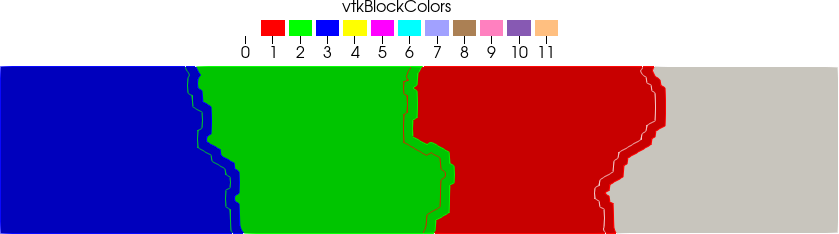
\includegraphics[align=t,width=1\textwidth]{./Images/2d-bar-partioned.png}
    \end{minipage}\hspace{.1\textwidth}
    \begin{minipage}[t][2cm][t]{0.4\textwidth}
    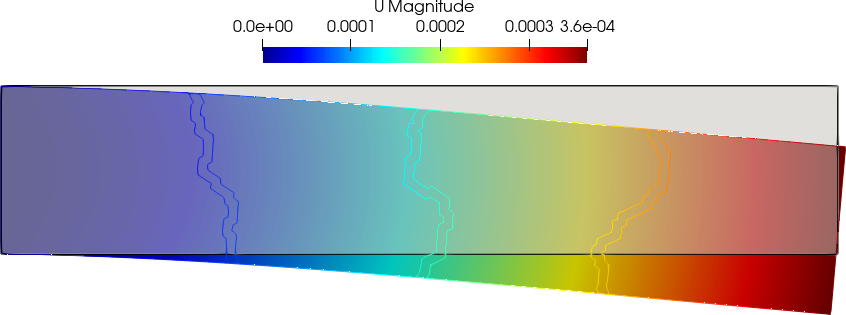
\includegraphics[align=t,width=1\textwidth]{./Images/2d-bar-results.png}
    \end{minipage}
    \caption{2D clamped bar results. Partitioned mesh (left) and 1000X warped displacement field (right).}
    \label{fig:2d-bar-results}
\end{figure}


\subsection{PSD simulation of 2D bar problem clamped at both ends \label{sec:2D-bar-clamped1}}

For this test the properties of the material are the same as used in \cref{sec:2d-bar-load}. 

\textbf{Step 1: Preprocessing}

For ``PSD preprocessing'' go to any folder, launch the terminal there and run the following command.
\begin{lstlisting}[style=BashInputStyle]
PSD_PreProcess -problem linear-elasticity -dimension 2 -bodyforceconditions 1 -dirichletconditions 2 -postprocess u
\end{lstlisting}
%
Since basic nature of both the problems is same this is the exact same command used in preprocessing of \cref{sec:2d-bar-load}. The only difference of this problem compared to the one from \cref{sec:2d-bar-load} is that an additional Dirichlet condition needs to be supplied, notified to PSD by {\ttfamily -dirichletconditions 2}. To provide Dirichlet conditions of the left clamped end ($u_x=u_y=0$) in {\ttfamily ControlParameters.edp} set {\ttfamily Dbc0On 2}, {\ttfamily Dbc0Ux 0.}, and {\ttfamily Dbc0Uy 0.}. Similarly, for the right end set variables {\ttfamily Dbc1On 4}, {\ttfamily Dbc1Ux 0.}, and {\ttfamily Dbc1Uy 0}. Each one of these is a clamped border respectively labeled as 2  ({\ttfamily Dbc0On 2}) and 4 ({\ttfamily Dbc1On 4}) in the mesh.

\textbf{Step 2: Solving}

Let us now use  3 cores to solve this problem. To do so enter the following command:

\begin{lstlisting}[style=BashInputStyle]
PSD_Solve -np 3 Main.edp
\end{lstlisting}
%
Notice, that this is the exact same command used in solving of \cref{sec:2d-bar-load}, with only difference that we now use {\ttfamily -np 3} vs.~{\ttfamily -np 4}.


\textbf{Step 3: Postprocessing}

Launch ParaView and have a look at the  {\ttfamily .pvd} file in the  {\ttfamily PSD/Solver/VTUs\_DATE\_TIME} folder. 

\begin{figure}[htbp]
    \centering
    \begin{minipage}[t][2cm][t]{0.4\textwidth}
    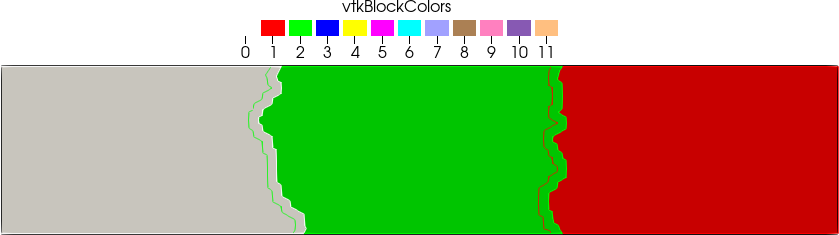
\includegraphics[align=t,width=1\textwidth]{./Images/2d-bar-partitioned3.png}
    \end{minipage}\hspace{.1\textwidth}
    \begin{minipage}[t][2cm][t]{0.4\textwidth}
    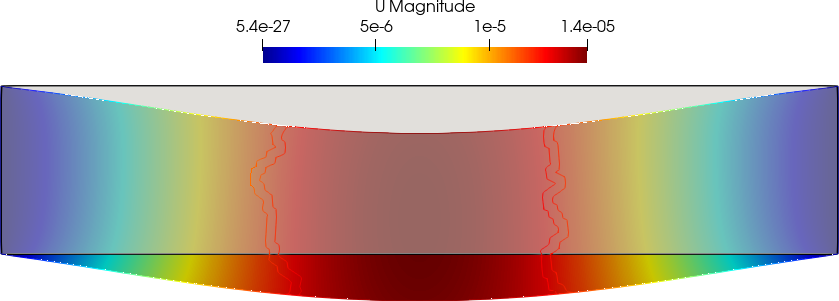
\includegraphics[align=t,width=1\textwidth]{./Images/2d-bar-clamped-ends.png}
    \end{minipage}
    \caption{2D clamped bar results. Partitioned mesh (left) and 20000X warped displacement field (right).}
    \label{fig:3part}
\end{figure}

In~\cref{fig:3part} there are only three subdomais in the partitioned mesh since only three cores were used.

\subsubsection{Redoing the test on Jupiter and moon}

Imagine, you wish to know how the test would compare if performed on Moon and Jupiter. The only thing that will change now is the gravitational pull, for Moon $g=1.32$ and for Jupiter $g=24.79$. To perform the moon test simply change  {\ttfamily Fbc0Fy -10560.0} in {\ttfamily ControlParameters.edp} and redo step 2 and step 3. Similarly, for the Jupiter test {\ttfamily Fbc0Fy -198320.0} in {\ttfamily ControlParameters.edp} and redo step 2 and step 3.

\begin{figure}[htbp]
    \centering
    \begin{minipage}[t][2.5cm][t]{0.4\textwidth}
    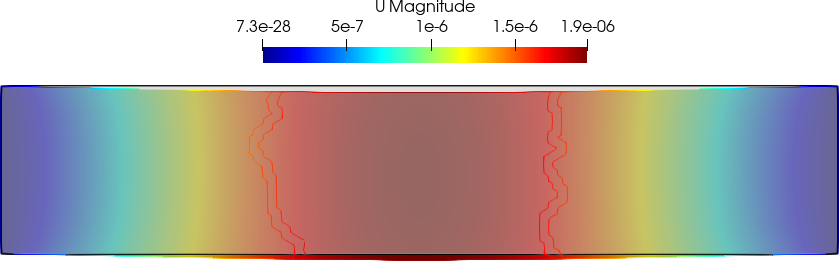
\includegraphics[align=t,width=1\textwidth]{./Images/2d-bar-moon.png}
    \end{minipage}\hspace{.1\textwidth}
    \begin{minipage}[t][2.5cm][t]{0.4\textwidth}
    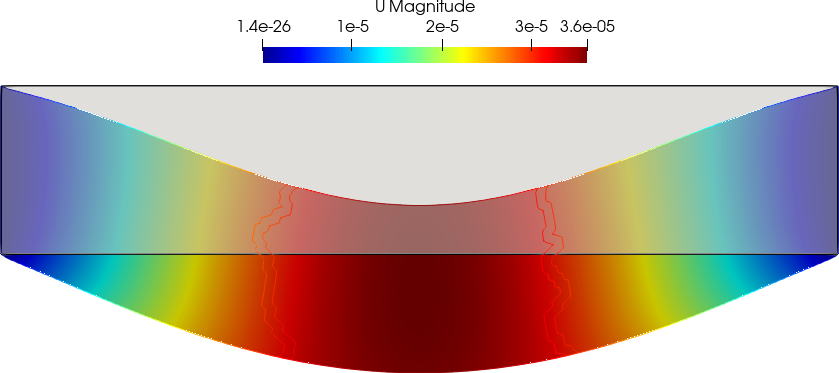
\includegraphics[align=t,width=1\textwidth]{./Images/2d-bar-Jupiter.png}
    \end{minipage}
    \caption{2D clamped bar 20000X warped displacement fields. On moon (left) and  on Jupiter (right).}
    \label{fig:moon-jupiter}
\end{figure}

\subsection{PSD simulation of 2D bar problem clamped at one end wile being pulled at the other end (Dirichlet-Dirichlet case)\label{sec:2d-bar-clamped2}}

In this section we showcase the 2D bar problem simulation with one end clamped wile being pulled at the other end. Body force is neglected and the non clamped ends pull is approximated with Dirichlet displacement $u_1=1$. If this simulation is compared to the previous one from \cref{sec:2d-bar-load}, the only difference now is that no body force is applied and an additional Dirichlet condition is applied at the free end of the bar. Here is how PSD simulation of this case can be performed.

\textbf{Step 1: Preprocessing}

For ``PSD preprocessing'' go to any folder, launch the terminal there and run the following command.
\begin{lstlisting}[style=BashInputStyle]
PSD_PreProcess -problem linear-elasticity -dimension 2 -dirichletconditions 2 -postprocess u
\end{lstlisting}
%
In comparison to preprocessing from \cref{sec:2d-bar-load,sec:2D-bar-clamped1}, notice that {\ttfamily -bodyforceconditions 1} is missing. This is due to the fact that for this problem we assume null body force. Just like in~\cref{sec:2D-bar-clamped1} {\ttfamily -dirichletconditions 2}, which notifies to PSD that there are two Dirichlet borders ---the clamped and the pulled ends of the bar--- in this simulation.
To provide these Dirichlet conditions of the two ends in {\ttfamily ControlParameters.edp} set the variables  {\ttfamily Dbc0On 2}, {\ttfamily Dbc0Ux 0.}, and {\ttfamily Dbc0Uy 0.} signifying the clamped end ($u_x=0,u_y=0$ on mesh label 2) and {\ttfamily Dbc1On 4}, {\ttfamily Dbc1Ux 1.}, and {\ttfamily Dbc1Uy 0.} signifying the pulled end ($u_x=1,u_y=0$  on label 4). Note that here at border 4 we have explicitly set $u_2=0$ this means the bar is not allowed to shrink(compress) in $y$ direction, however you might wish to allow the bar to compress. For such a simulation simply use {\ttfamily Dbc1On 4} and {\ttfamily Dbc1Ux 1.}, and remove the term {\ttfamily Dbc1Uy 0.} therefor asking PSD not to apply constrain in $y$ direction on the pulled end.

\textbf{Step 2: Solving}

Let us now use 2 cores to solve this problem. To do so enter the following command:

\begin{lstlisting}[style=BashInputStyle]
PSD_Solve -np 2 Main.edp
\end{lstlisting}
%
Notice, that this is the exact same command used in solving of \cref{sec:2d-bar-load,sec:2D-bar-clamped1}, with only difference that we now use {\ttfamily -np 2} vs.~{\ttfamily -np 4} in \cref{sec:2d-bar-load} and ~{\ttfamily -np 3} in \cref{sec:2D-bar-clamped1}.


\textbf{Step 3: Postprocessing}

Launch ParaView and have a look at the  {\ttfamily .pvd} file in the  {\ttfamily PSD/Solver/VTUs\_DATE\_TIME} folder. 

\begin{figure}[htbp]
    \centering
    \begin{minipage}[t][2cm][t]{0.39\textwidth}
    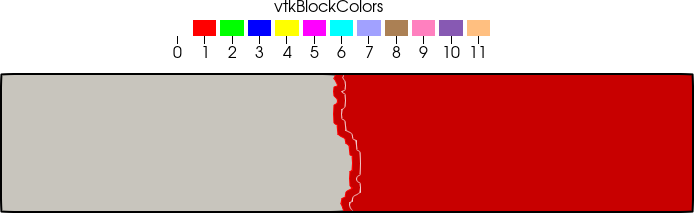
\includegraphics[align=t,width=1\textwidth]{./Images/2d-bar-clamped-pulled-partioned.png}
    \end{minipage}\hspace{.1\textwidth}
    \begin{minipage}[t][2cm][t]{0.5\textwidth}
    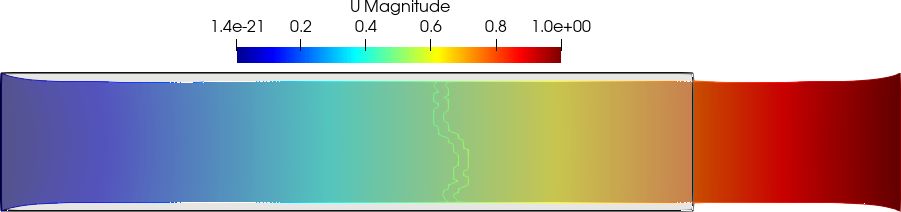
\includegraphics[align=t,width=1\textwidth]{./Images/2d-bar-clamped-pulled.png}
    \end{minipage}
    \caption{2D bar results. Partitioned mesh (left) and 1.5X warped displacement field (right).}
    \label{fig:2part}
\end{figure}

Note now in~\cref{fig:2part} there are only two subdomais in the partitioned mesh since only three cores were used. As expected we see that the right end of the bar which is being pulled does not contract in $y$ direction.
\pagebreak


\subsection{PSD simulation of 2D bar problem clamped at one end wile being pulled at the other end (Dirichlet--Neumann case)\label{sec:2d-bar-clamped3}}


Similar simulation, as in \cref{sec:2d-bar-clamped2} is presented in this section. We showcase the 2D bar problem simulation with one end clamped wile being pulled at the other end. Just like simulation from \cref{sec:2d-bar-clamped2} the body force is neglected, However now  the non clamped ends pull is approximated with Neumann force $\int_{\partial\Omega^h_{\text N}}(\mathbf t\cdot \bvh)$. To simulate the pull we assume traction vector $\mathbf t=[t_x,t_y]=[10^9.,0]$ acting on the non clamped right end of the bar, i.e., force in $x$ direction is 10 units. Here is how PSD simulation of this case can be performed.

\textbf{Step 1: Preprocessing}

For ``PSD preprocessing'' go to any folder, launch the terminal there and run the following command.
\begin{lstlisting}[style=BashInputStyle]
PSD_PreProcess -problem linear-elasticity -dimension 2 -dirichletconditions 1 -tractionconditions 1 -postprocess u
\end{lstlisting}
%
the comandline flag {\ttfamily -dirichletconditions 1}, notifies to PSD that there is one Dirichlet border ---the clamped end of the bar--- in this simulation. And the flag {\ttfamily -tractionconditions 1} notifies to PSD that there is one traction border ---the right end of the bar--- in this simulation. 
To provide the clamped boundary condition ($u_1=0,u_2=0$) set the variables  {\ttfamily Dbc0On 2}, {\ttfamily Dbc0Ux 0.}, and {\ttfamily Dbc0Uy 0.} in {\ttfamily ControlParameters.edp}. In the same file traction boundary conditions are provided via the variables {\ttfamily Tbc0On 4} and {\ttfamily Tbc0Tx 1.e9}, which mean apply traction force $\mathbf t=[t_x,t_y]=[10^9.,0]$ on label number 4 (right) of the mesh. If user wishes to add traction force ,for instance $t_y=100.$, simply add the missing macro {\ttfamily macro Tbc0Tx 1.e9 //}.


\textbf{Step 2: Solving}

Let us now use 5 cores to solve this problem. To do so enter the following command:

\begin{lstlisting}[style=BashInputStyle]
PSD_Solve -np 5 Main.edp
\end{lstlisting}
%
Notice, that this is the exact same command used in solving the previous bar problems from other sections, with only difference that we now use {\ttfamily -np 5}.


\textbf{Step 3: Postprocessing}

Launch ParaView and have a look at the  {\ttfamily .pvd} file in the  {\ttfamily PSD/Solver/VTUs\_DATE\_TIME} folder. 

\begin{figure}[htbp]
    \centering
    \begin{minipage}[t][2cm][t]{0.36\textwidth}
    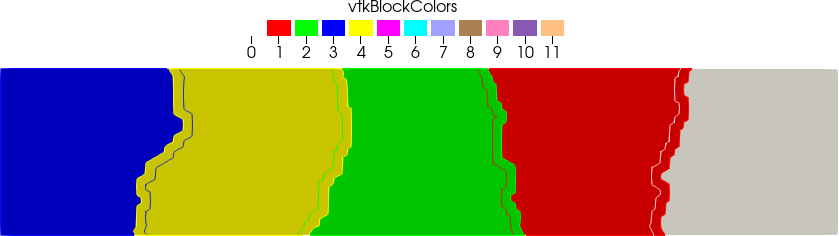
\includegraphics[align=b,width=1\textwidth]{./Images/2d-bar-partitioned5.png}
    \end{minipage}\hspace{.1\textwidth}
    \begin{minipage}[t][2cm][t]{0.5\textwidth}
    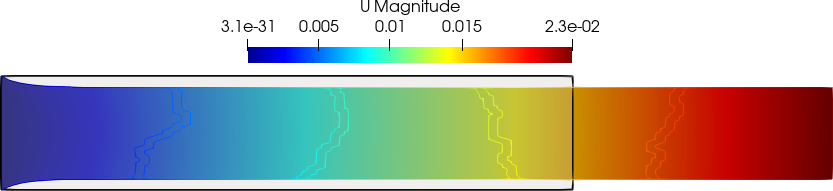
\includegraphics[align=b,width=1\textwidth]{./Images/2d-bar-clamped-traction.png}
    \end{minipage}
    \caption{2D bar results. Partitioned mesh (left) and 100X warped displacement field (right).}
    \label{fig:5part}
\end{figure}

Note now in~\cref{fig:5part} there are five subdomains in the partitioned mesh since five cores were used. Contrary to~\cref{fig:2part}, as expected, we see that the right end of the bar which is being pulled now contract in $y$ direction. This is due to the fact that there is no Dirichlet condition at this end now. 

\pagebreak




\subsection{PSD simulation of 2D bar problem clamped at one end wile being pulled at the other end (Dirichlet-Neumann-Point boundary conditions case)\label{sec:2d-bar-clamped4}}


Similar simulations, as in \cref{sec:2d-bar-clamped2,sec:2d-bar-clamped3} is presented in this section. We showcase the 2D bar problem simulation with one end clamped  wile being pulled at the other end. Contrary to simulation in \cref{sec:2d-bar-clamped2,sec:2d-bar-clamped3}, the clamped end just restricts $x$ movement, i.e, $u_x=0$. Just like simulation from \cref{sec:2d-bar-clamped2,sec:2d-bar-clamped3} the body force is neglected. Just like simulation in  \cref{sec:2d-bar-clamped3}, the non clamped ends pull is approximated with Neumann force $\int_{\partial\Omega^h_{\text N}}(\mathbf t\cdot \bvh)$. To simulate the pull we assume traction vector $\mathbf t=[t_x,t_y]=[10^9,0]$ acting on the non clamped right end of the bar, i.e., force in $x$ direction is $10^9$ units. Here is how PSD simulation of this case can be performed.


\textbf{Step 1: Preprocessing}

For ``PSD preprocessing'' go to any folder, launch the terminal there and run the following command.
\begin{lstlisting}[style=BashInputStyle]
PSD_PreProcess -problem linear-elasticity -dimension 2 -dirichletconditions 1 -tractionconditions 1 \
-dirichletpointconditions 1 -postprocess u
\end{lstlisting}

Additional flag {\ttfamily -dirichletpointconditions 1} now appears, this notifies to PSD that there is one Dirichlet point boundary condition. Edit the  {\ttfamily ControlParameters.edp} to communicate the desired point boundary conditions, set the variables {\ttfamily Pbc0Ux  0.} and {\ttfamily Pbc0Uy  0.} to specify $u_x=0,u_y=0$, and variable {\ttfamily PbcCord = [[  0. , 0. ]];} to specify the point coordinates $(x,y)=(0,0)$. Via the flags we specified that {\ttfamily -dirichletconditions 1}, i.e., there is one Dirichlet border.
To provide the Dirichlet condition ($u_x=0$) set the variables {\ttfamily Dbc0On 2} and {\ttfamily Dbc0Ux 0.}  in {\ttfamily ControlParameters.edp}. PSD understands that 4 is the mesh border label on which Dirichlet is applied and ($u_x=0$) is the condition to be applied.

\textbf{Step 2: Solving}

Let us now use 6 cores to solve this problem. To do so enter the following command:

\begin{lstlisting}[style=BashInputStyle]
PSD_Solve -np 6 Main.edp
\end{lstlisting}
%
Notice, that this is the exact same command used in solving the previous bar problems from other sections, with only difference that we now use {\ttfamily -np 6}.


\textbf{Step 3: Postprocessing}

Launch ParaView and have a look at the  {\ttfamily .pvd} file in the  {\ttfamily PSD/Solver/VTUs\_DATE\_TIME} folder. 

\begin{figure}[htbp]
    \centering
    \begin{minipage}[t][2cm][t]{0.36\textwidth}
    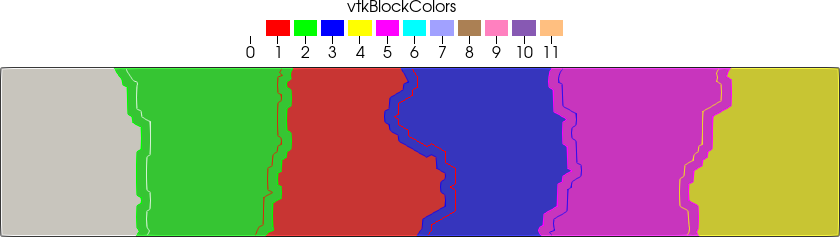
\includegraphics[align=b,width=1\textwidth]{./Images/2d-bar-partitioned6.png}
    \end{minipage}\hspace{.1\textwidth}
    \begin{minipage}[t][2cm][t]{0.5\textwidth}
    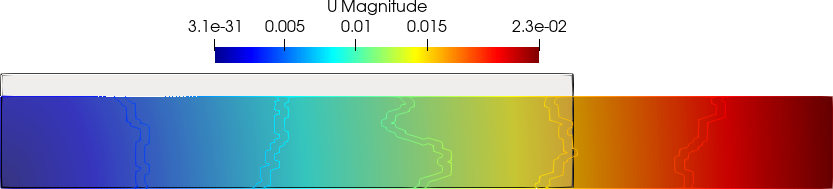
\includegraphics[align=b,width=1\textwidth]{./Images/2d-bar-clamped-traction-point.png}
    \end{minipage}
    \caption{2D bar results. Partitioned mesh (left) and 100X warped displacement field (right).}
    \label{fig:6part}
\end{figure}

Note now in~\cref{fig:6part} there are six subdomais in the partitioned mesh. As expected, we see that the right and the left end of the bar which is being pulled now contract in $y$ direction, and the bar elongates in $x$ direction. 


\pagebreak



\subsection{PSD simulation of 3D bar problem clamped at one end wile being pulled at the other end (Dirichlet-Neumann case)\label{sec:3d-bar-clamped3}}

In this section we present a 3D PSD simulation of a clamped bar which his being loaded in vertical direction at the non-clamped end. This simulation is like the one presented in \cref{sec:2d-bar-clamped3}, however in 3D. The material properties are same as before, and at the non-clamped end traction $t_y=-10^9$ units. The 3D bar is $1\times1\times5$ m$^3$.

Here is how PSD simulation of this case can be performed.

\textbf{Step 1: Preprocessing}

For ``PSD setup'' go to any folder, launch the terminal there and run the following command.
\begin{lstlisting}[style=BashInputStyle]
PSD_PreProcess  -problem linear-elasticity -dimension 3 -dirichletconditions 1 -tractionconditions 1 -postprocess u
\end{lstlisting}
%
the comandline flag {\ttfamily -dirichletconditions 1} notifies to PSD that there is one Dirichlet border ---the clamped end of the bar--- in this simulation; {\ttfamily -dimension 3} means the simulation is 3D. And the flag {\ttfamily -tractionconditions 1} notifies to PSD that there is one traction border ---the right end of the bar--- in this simulation. 
To provide Dirichlet conditions of the  clamped end ($u_x=0,u_y=0,u_z=0$) in {\ttfamily ControlParameters.edp} set {\ttfamily Dbc0On 1}, {\ttfamily Dbc0Ux 0.}, {\ttfamily Dbc0Uy 0.}, and {\ttfamily Dbc0Uz 0.}, where 1 being the surface mesh label of the clamped end. To add the traction boundary condition set  {\ttfamily Tbc0On 2} and {\ttfamily Tbc0Ty -1.e9}, here the mesh label number of the right end is 2. For this end $\mathbf t=[t_x,t_y,t_z]=[0.,10^9,0.]$, hence in {\ttfamily ControlParameters.edp} we only  use {\ttfamily Tbc0Ty -1.e9}. 


\textbf{Step 2: Solving}

Let us now use 4 cores to solve this problem. To do so enter the following command:

\begin{lstlisting}[style=BashInputStyle]
PSD_Solve -np 4 Main.edp
\end{lstlisting}
%
Notice, that this is the exact same command used in solving the previous bar problems from other sections.


\textbf{Step 3: Postprocessing}

Launch ParaView and have a look at the  {\ttfamily .pvd} file in the  {\ttfamily PSD/Solver/VTUs\_DATE\_TIME} folder. 

\begin{figure}[htbp]
    \centering
    \begin{minipage}[t][2cm][t]{0.38\textwidth}
    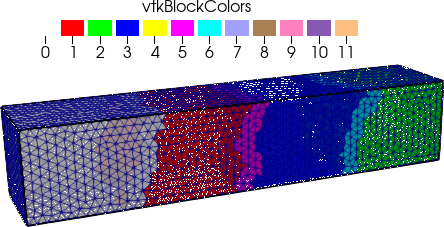
\includegraphics[align=b,width=1\textwidth]{./Images/3d-bar-clamped-ends.png}
    \end{minipage}\hspace{.1\textwidth}
    \begin{minipage}[t][2cm][t]{0.4\textwidth}
    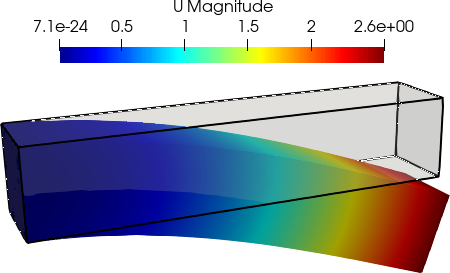
\includegraphics[align=b,width=1\textwidth]{./Images/3d-bar-clamped-pulled-partioned.png}
    \end{minipage}
    \caption{3D bar results. Partitioned mesh (left) and 0.5X warped displacement field (right).}
    \label{fig:3Dpart}
\end{figure}

In~\cref{fig:3Dpart} there are four subdomais in the partitioned mesh since four cores were used.

\pagebreak


\subsection{PSD simulation of 3D  mechanical piece (Dirichlet-Neumann case) with complex mesh\label{sec:3d-bar-clamped3-sub}}

So far in the previous cases we only concentrated on bar simulations, which were more or less trivial cases. Moreover, the bar meshes are provided with the PSD solver. In this section we now turn towards  3D simulation of a mechanical piece, the geometry of which is shown in~\cref{fig:mechanicalpiecegeo}. The left (small) hole is fixed: $u_1=u_2=u_3=0$, while as traction force $t_x=10^9$ is applied on the large hole.

You can grab a copy of CAD geometry for the mechanical piece (the Gmsh {\ttfamily .geo}) your local Gmsh installation folder  {\ttfamily gmsh/share/doc/gmsh/demos/simple\_geo/{piece}.geo}. The listing of the file is also given in @. To generate the mesh {\ttfamily piece.msh} simply do 
\begin{lstlisting}[style=BashInputStyle]
gmsh -3 piece.geo
\end{lstlisting}
Place the generated mesh {\ttfamily piece.msh} in {\ttfamily /PSD/Meshes/3D/piece.msh}. Now the PSD simulation can be performed.

\begin{figure}[h]
    \centering
    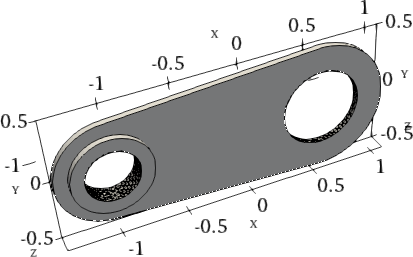
\includegraphics[align=b,width=0.5\textwidth]{./Images/3d-mechanical.png}
    \caption{3D mechanical piece.}
    \label{fig:mechanicalpiecegeo}
\end{figure}

\textbf{Step 1: Preprocessing}

For ``PSD setup'' go to any folder, launch the terminal there and run the following command.
\begin{lstlisting}[style=BashInputStyle]
PSD_PreProcess  -problem linear-elasticity -dimension 3 -dirichletconditions 1 -tractionconditions 1 -postprocess u
\end{lstlisting}
Here, by using these parameters we have generated one Dirichlet condition and one traction condition, respectively to be applied to the small and the large holes in the mesh. Further, by using {\ttfamily -dimension 3} we have let PSD know that the problem is 3D .In the {\ttfamily /PSD/Meshes/3D/piece.msh} generated, the label 4 (resp.~3) corresponds to the Dirichlet (resp.~traction) border. 
To provide Dirichlet conditions on label number 4 ($u_x=0,u_y=0,u_z=0$) in {\ttfamily ControlParameters.edp} use set {\ttfamily Dbc0On 4}, {\ttfamily Dbc0Ux 0.}, {\ttfamily Dbc0Uy 0.}, and {\ttfamily Dbc0Uz 0.}. To add the values and label numbers of the traction borders edit the  {\ttfamily ControlParameters.edp}, set  {\ttfamily Tbc0On 3} and {\ttfamily Tbc0Ty -1.e9}. For this end $\mathbf t=[t_x,t_y,t_z]=[0.,10^9,0.]$. Finally we use steel properties for the material, so in {\ttfamily ControlParameters.edp} the parameters {\ttfamily real E  = 200.e9;} and {\ttfamily real nu = 0.3;} should be used. These represent $E$ and $\nu$, respectively. With all the properties and boundary conditions set we now use  {\ttfamily string ThName = "../Meshes/3D/piece";} in the {\ttfamily ControlParameters.edp} file, this notifies PSD about the name of the mesh used for this simulation.  

\textbf{Step 2: Solving}

Let us now use 2 cores to solve this problem. To do so enter the following command:

\begin{lstlisting}[style=BashInputStyle]
PSD_Solve -np 2 Main.edp
\end{lstlisting}

\textbf{Step 3: Postprocessing}

Launch ParaView and have a look at the  {\ttfamily .pvd} file in the  {\ttfamily PSD/Solver/VTUs\_DATE\_TIME} folder. 

\begin{figure}[htbp]
    \centering
    \begin{minipage}[t][2cm][t]{0.36\textwidth}
    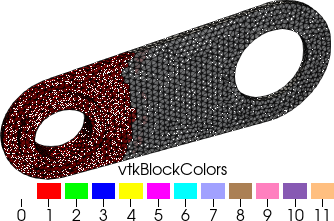
\includegraphics[align=b,width=1\textwidth]{./Images/3d-mechanical-part.png}
    \end{minipage}\hspace{.1\textwidth}
    \begin{minipage}[t][2cm][t]{0.4\textwidth}
    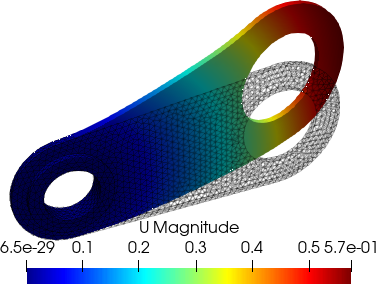
\includegraphics[align=b,width=1\textwidth]{./Images/3d-mechanical-result.png}
    \end{minipage}
    \caption{Mechanical piece test results. Partitioned mesh (left) and  warped displacement field (right).}
    \label{fig:mechapieceresult}
\end{figure}

\textbf{Redoing the test with different conditions}

\begin{figure}[htbp]
    \centering
    \begin{minipage}{0.42\textwidth}
    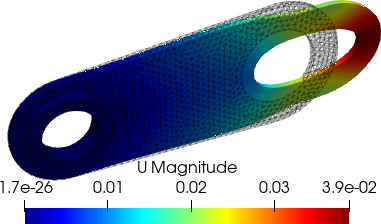
\includegraphics[align=b,width=1\textwidth]{./Images/3d-mechanical-result-x.png}
    \subcaption{{\ttfamily real  tx0=1.e9, ty0=0, tz0=0.,;}}
    \end{minipage}\hspace{.1\textwidth}
    \begin{minipage}{0.4\textwidth}
    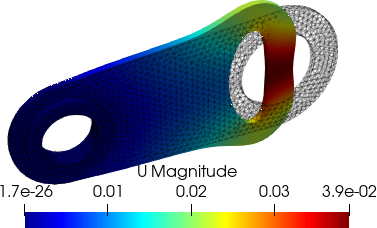
\includegraphics[align=b,width=1\textwidth]{./Images/3d-mechanical-result--x.png}
    \subcaption{{\ttfamily real  tx0=1.e9, ty0=0, tz0=0.,;}}
    \end{minipage}
    \caption{Mechanical piece test results.}
    \label{fig:mechapieceresult2}
\end{figure}



\pagebreak













\section{Damage mechanics}
\subsection{Hybrid phase-field for damage}
On a meshed domain $\Omega^h\in\Omega\subset\mathbb{R}^n$, for damage mechanics the mixed finite element variational formulation in the Lagrangian framework for searching the unknown nodal displacements vector $\bu^h=[u_1,u_2,u_3]^\mathsf{T}$ reads,
%
%
\begin{equation}\label{Eq:VarfU}
\begin{aligned}
&\text{search}~\buh\in\mathbb{V}^h \text{~that satisfies}~\forall\, t\in[0,T]:\\
&\int_{\Omega^h}\big[(1-d^h)^2 + \kappa \big]\sig(\buh) : \eps(\bvh) \,\dv= \int_{\partial\Omega^h_\text{N}} \overline{\bt}\cdot\bvh \,\ds \quad\forall\,\bv^h\in\mathbb{V}^h,
\end{aligned}
\end{equation}
where $\kappa\ll1$ is a model parameter to prevent numerical singularity when $d \to 1$.
 %
 %
In this formulation, the notation ``$:$'' is used for the double contraction between tensors (i.e., component-wise tensor product) and $ \mathbb{V}^h $ is a  mixed third order vector valued finite element functional space to approximate vector test function~$\bvh$ and vector trial function~$\buh$:
 %
\begin{equation}
\mathbb{V}^h=\left\{ \bu^h\in [ {H}^1(\Omega^h) ]^3~~\forall t\in[0,T]~|~ \forall \bx\in\partial\Omega^h_{\text{D}}~\buh=\overline{\bu}\right\},
\end{equation}
%
with ${H}^1(\Omega^h)$ denoting a square integrable Sobolev functional space.
Similarly, for~the phase-field the standard finite element variational formulation for the unknown damage scalar $\fih$ reads, 
%
%
\begin{equation}
\begin{aligned}\label{Eq:VarfPhi}
&\text{search}~\fih\in{{V}}^h \text{~that satisfies}~\forall\, t\in[0,T]:\\
&\int_{\Omega^h}\left[ \frac{\bgc}{l_0} + 2 \mathcal{H}^{+}(\buh) \right]\fih\ttah\, \dv + \int_{\Omega^h} {\bgc}{l_0}\nabla\fih \cdot \nabla\ttah \, \dv= \int_{\Omega^h} 2\mathcal{H}^{+}(\buh)\ttah \, \dv\quad\forall\,\ttah\in{{V}}^h, 
\end{aligned}
\end{equation}
%
%
where,~${{V}}^h$ denotes the scalar finite element functional space to approximate scalar test function~$\ttah$ and scalar trial function~$\fih$:
\begin{equation}
{{V}}^h=\left\{\fih \in  {H}^1(\Omega^h)~~\forall t\in[0,T]~\middle|~\fih\in[0,1]  \right\}.
\end{equation}

\pagebreak

\section{Elastodynamics}
\pagebreak

\section{Soil dynamics}



\pagebreak

\section{General list of examples: Linear Elasticity}
 *============================================================*\\
  \textbf{Sequential  2D linear-elasticity}\\                   
 *============================================================*\\
\begin{lstlisting}[style=BashInputStyle] 
PSD_PreProcess -dimension 2 -bodyforceconditions 1 conditions 1 -sequential -dirichletconditions 1 
	
PSD_Solve_Seq Main.edp -v 0 -ns -nw 
\end{lstlisting}


*============================================================*\\
 \textbf{Sequential  3D linear-elasticity}                   \\
*============================================================*\\
\begin{lstlisting}[style=BashInputStyle] 
PSD_PreProcess -dimension 3 -bodyforceconditions 1 -sequential -dirichletconditions 1

PSD_Solve_Seq Main.edp -v 0 -ns -nw
\end{lstlisting}


*============================================================*\\
\textbf{ Sequential  2D linear-elasticity fastmethod }      \\
*============================================================*\\
\begin{lstlisting}[style=BashInputStyle] 
PSD_PreProcess -dimension 2 -bodyforceconditions 1 -sequential -dirichletconditions 1 -fastmethod 

PSD_Solve_Seq Main.edp -v 0 -ns -nw	
\end{lstlisting}
*============================================================*\\
\textbf{ Sequential  3D linear-elasticity   fastmethod }     \\
*============================================================*\\
\begin{lstlisting}[style=BashInputStyle] 
PSD_PreProcess -dimension 3 -bodyforceconditions 1 -sequential -dirichletconditions 1 -fastmethod 

PSD_Solve_Seq Main.edp -v 0 -ns -nw  	
\end{lstlisting}



*============================================================*\\
\textbf{ Parallel 2D linear-elasticity }                  \\
*============================================================*\\
	
\begin{lstlisting}[style=BashInputStyle]
PSD_PreProcess -dimension 2 -bodyforceconditions 1  -dirichletconditions 1 

ff-mpirun-np 2  Main.edp -v 0 -ns -nw
\end{lstlisting}
*============================================================\\
\textbf{ Parallel 3D linear-elasticity  }                 \\
*============================================================\\
	
\begin{lstlisting}[style=BashInputStyle]
PSD_PreProcess -dimension 3 -bodyforceconditions 1  -dirichletconditions 1 

ff-mpirun-np 2  Main.edp -v 0 -ns -nw
\end{lstlisting}
*============================================================\\
\textbf{ Parallel 2D linear-elasticity     fastmethod  }            \\
*============================================================\\
	
\begin{lstlisting}[style=BashInputStyle]
PSD_PreProcess -dimension 2 -bodyforceconditions 1  -dirichletconditions 1 -fastmethod  

ff-mpirun-np 2  Main.edp -v 0 -ns -nw	
\end{lstlisting}
*============================================================\\
\textbf{ Parallel 3D linear-elasticity     fastmethod }             \\
*============================================================\\
	
\begin{lstlisting}[style=BashInputStyle]
PSD_PreProcess -dimension 3 -bodyforceconditions 1  -dirichletconditions 1 -fastmethod  

ff-mpirun-np 2  Main.edp -v 0 -ns -nw
\end{lstlisting}

\section{General list of examples: Fracture mechanics}

*============================================================\\
\textbf{ Sequential  2D phase-field fracture mechanics }\\
*============================================================\\
\begin{lstlisting}[style=BashInputStyle]
PSD_PreProcess -dimension 2 -problem damage -model hybrid-phase-field -sequential -dirichletconditions 2   

PSD_Solve Main.edp -v 0 -ns -nw   
\end{lstlisting}
*============================================================\\
\textbf{ Sequential  3D phase-field fracture mechanics}\\ 
*============================================================\\

\begin{lstlisting}[style=BashInputStyle]
PSD_PreProcess -dimension 3 -problem damage -model hybrid-phase-field -sequential -dirichletconditions 2   

PSD_Solve Main.edp -v 0 -ns -nw   
\end{lstlisting}
*============================================================\\
\textbf{ Parallel 2D phase-field fracture mechanics} \\
*============================================================\\

\begin{lstlisting}[style=BashInputStyle]
PSD_PreProcess -dimension 2 -problem damage -model hybrid-phase-field -dirichletconditions 2   

PSD_Solve -np 2  Main.edp -v 0 -ns -nw   
\end{lstlisting}
*============================================================\\
\textbf{ Parallel 3D phase-field fracture mechanics} \\
*============================================================\\
\begin{lstlisting}[style=BashInputStyle]
PSD_PreProcess -dimension 3 -problem damage -model hybrid-phase-field -dirichletconditions 2   

PSD_Solve -np 2  Main.edp -v 0 -ns -nw   
\end{lstlisting}
*============================================================\\
\textbf{ Parallel 2D phase-field fracture mechanics with vectorial FEM } \\
*============================================================\\

\begin{lstlisting}[style=BashInputStyle]
PSD_PreProcess -dimension 2 -problem damage -model hybrid-phase-field -vectorial -dirichletconditions 2   

PSD_Solve -np 2  Main.edp -v 0 -ns -nw   
\end{lstlisting}
*============================================================\\
\textbf{ Parallel 3D phase-field fracture mechanics  with vectorial FEM} \\
*============================================================\\
\begin{lstlisting}[style=BashInputStyle]
PSD_PreProcess -dimension 3 -problem damage -model hybrid-phase-field -vectorial -dirichletconditions 2   

PSD_Solve -np 2  Main.edp -v 0 -ns -nw   
\end{lstlisting}
*============================================================\\
\textbf{ Sequential 2D  phase-field fracture mechanics energydecomp }\\
*============================================================\\
\begin{lstlisting}[style=BashInputStyle]
PSD_PreProcess -dimension 2 -problem damage -model hybrid-phase-field -sequential -dirichletconditions 2 \
-energydecomp   

PSD_Solve_Seq Main.edp -v 0 -ns -nw   
\end{lstlisting}
*============================================================\\
\textbf{ Sequential 3D phase-field fracture mechanics energydecomp }\\
*============================================================\\
\begin{lstlisting}[style=BashInputStyle]
PSD_PreProcess -dimension 3 -problem damage -model hybrid-phase-field -sequential -dirichletconditions 2 \
-energydecomp   

PSD_Solve_Seq Main.edp -v 0 -ns -nw   
\end{lstlisting}
*============================================================\\
\textbf{ Parallel 2D phase-field fracture mechanics energydecomp }\\
*============================================================\\
\begin{lstlisting}[style=BashInputStyle]
PSD_PreProcess -dimension 2 -problem damage -model hybrid-phase-field -dirichletconditions 2 -energydecomp   

PSD_Solve -np 2  Main.edp -v 0 -ns -nw   
\end{lstlisting}
*============================================================\\
\textbf{ Parallel 3D phase-field fracture mechanics energydecomp }\\
*============================================================\\
\begin{lstlisting}[style=BashInputStyle]
PSD_PreProcess -dimension 3 -problem damage -model hybrid-phase-field -dirichletconditions 2 -energydecomp   

PSD_Solve -np 2  Main.edp -v 0 -ns -nw   
\end{lstlisting}
*============================================================\\
\textbf{ Parallel 2D phase-field fracture mechanics energydecomp \& vectorial}\\
*============================================================\\
\begin{lstlisting}[style=BashInputStyle]
PSD_PreProcess -dimension 2 -problem damage -model hybrid-phase-field -vectorial -dirichletconditions 2 \
-energydecomp   

PSD_Solve -np 2  Main.edp -v 0 -ns -nw   
\end{lstlisting}
*============================================================\\
\textbf{ Parallel 3D phase-field fracture mechanics energydecomp }\\
*============================================================\\
\begin{lstlisting}[style=BashInputStyle]
PSD_PreProcess -dimension 3 -problem damage -model hybrid-phase-field -vectorial -dirichletconditions 2 \
-energydecomp   

PSD_Solve -np 2  Main.edp -v 0 -ns -nw   
\end{lstlisting}
*============================================================\\
\textbf{ Sequential 2D phase-field fracture mechanics with GFP }\\
*============================================================\\
\begin{lstlisting}[style=BashInputStyle]
PSD_PreProcess -dimension 2 -problem damage -model hybrid-phase-field  -dirichletconditions 2 \
-sequential -useGFP   

PSD_Solve Main.edp -v 0 -ns -nw   
\end{lstlisting}
*============================================================\\
\textbf{ Sequential 3D phase-field fracture mechanics with GFP} \\
*============================================================\\
\begin{lstlisting}[style=BashInputStyle]
PSD_PreProcess -dimension 3 -problem damage -model hybrid-phase-field  -dirichletconditions 2 \
-sequential -useGFP   

PSD_Solve Main.edp -v 0 -ns -nw   
\end{lstlisting}
*============================================================\\
\textbf{ Parallel 2D phase-field fracture mechanics with GFP} \\
*============================================================\\
\begin{lstlisting}[style=BashInputStyle]
PSD_PreProcess -dimension 2 -problem damage -model hybrid-phase-field -dirichletconditions 2 -useGFP   

PSD_Solve -np 2  Main.edp -v 0 -ns -nw   
\end{lstlisting}
*============================================================\\
\textbf{ Parallel 3D phase-field fracture mechanics with GFP }\\
*============================================================\\
\begin{lstlisting}[style=BashInputStyle]
PSD_PreProcess -dimension 3 -problem damage -model hybrid-phase-field -dirichletconditions 2 -useGFP   

PSD_Solve -np 2  Main.edp -v 0 -ns -nw   
\end{lstlisting}
*============================================================\\
\textbf{ Parallel 2D phase-field fracture mechanics with GFP \& vectorial} \\
*============================================================\\
\begin{lstlisting}[style=BashInputStyle]
PSD_PreProcess -dimension 2 -problem damage -model hybrid-phase-field -vectorial -dirichletconditions 2 -useGFP   

PSD_Solve -np 2  Main.edp -v 0 -ns -nw   
\end{lstlisting}
*============================================================\\
\textbf{ Parallel 3D phase-field fracture mechanics with GFP \& vectorial }\\
*============================================================\\
\begin{lstlisting}[style=BashInputStyle]
PSD_PreProcess -dimension 3 -problem damage -model hybrid-phase-field -vectorial -dirichletconditions 2 -useGFP   

PSD_Solve -np 2  Main.edp -v 0 -ns -nw   
\end{lstlisting}
*============================================================\\
 \textbf{Sequential 2D phase-field fracture mechanics with energydecomp \& GFP} \\
*============================================================\\
\begin{lstlisting}[style=BashInputStyle]
PSD_PreProcess -dimension 2 -problem damage -model hybrid-phase-field -sequential -dirichletconditions 2 \
-energydecomp -useGFP   

PSD_Solve Main.edp -v 0 -ns -nw   
\end{lstlisting}
*============================================================\\
\textbf{ Sequential 3D phase-field fracture mechanics with energydecomp \& GFP} \\
*============================================================\\
\begin{lstlisting}[style=BashInputStyle]
PSD_PreProcess -dimension 3 -problem damage -model hybrid-phase-field -sequential -dirichletconditions 2 \
-energydecomp -useGFP   

PSD_Solve_Seq Main.edp -v 0 -ns -nw   
\end{lstlisting}
*============================================================\\
 \textbf{Parallel 2D phase-field fracture mechanics with energydecomp \& GFP} \\
*============================================================\\
\begin{lstlisting}[style=BashInputStyle]
PSD_PreProcess -dimension 2 -problem damage -model hybrid-phase-field -dirichletconditions 2 \
-energydecomp -useGFP  

PSD_Solve -np 2  Main.edp -v 0 -ns -nw   
\end{lstlisting}
*============================================================\\
\textbf{ Parallel 3D phase-field fracture mechanics with energydecomp \& GFP} \\
*============================================================\\
\begin{lstlisting}[style=BashInputStyle]
PSD_PreProcess -dimension 3 -problem damage -model hybrid-phase-field -dirichletconditions 2 \
-energydecomp -useGFP   

PSD_Solve -np 2  Main.edp -v 0 -ns -nw   	
\end{lstlisting}
*============================================================\\
 \textbf{Parallel 2D phase-field fracture mechanics with energydecomp, vectorial \& GFP} \\
*============================================================\\
\begin{lstlisting}[style=BashInputStyle]
PSD_PreProcess -dimension 2 -problem damage -model hybrid-phase-field -vectorial -dirichletconditions 2 \
-energydecomp -useGFP  

PSD_Solve -np 2  Main.edp -v 0 -ns -nw   
\end{lstlisting}
*============================================================\\
\textbf{ Parallel 3D phase-field fracture mechanics with energydecomp, vectorial \& GFP} \\
*============================================================\\
\begin{lstlisting}[style=BashInputStyle]
PSD_PreProcess -dimension 3 -problem damage -model hybrid-phase-field -vectorial -dirichletconditions 2 \
-energydecomp -useGFP   

PSD_Solve -np 2  Main.edp -v 0 -ns -nw   	
\end{lstlisting}
*============================================================\\
 \textbf{Parallel 2D phase-field fracture mechanics with reaction-force, energydecomp, vectorial \& GFP} \\
*============================================================\\
\begin{lstlisting}[style=BashInputStyle]
PSD_PreProcess -dimension 2 -problem damage -model hybrid-phase-field -vectorial -dirichletconditions 2 \
-getreactionforce -energydecomp -useGFP  

PSD_Solve -np 2  Main.edp -v 0 -ns -nw   
\end{lstlisting}
*============================================================\\
\textbf{ Parallel 3D phase-field fracture mechanics with reaction-force, energydecomp, vectorial \& GFP} \\
*============================================================\\
\begin{lstlisting}[style=BashInputStyle]
PSD_PreProcess -dimension 3 -problem damage -model hybrid-phase-field -vectorial -dirichletconditions 2 \
-getreactionforce -energydecomp -useGFP   

PSD_Solve -np 2  Main.edp -v 0 -ns -nw   	
\end{lstlisting}
*============================================================\\
 \textbf{Parallel 2D phase-field fracture mechanics with live reaction-force plotting, energydecomp, vectorial \& GFP} \\
*============================================================\\
\begin{lstlisting}[style=BashInputStyle]
PSD_PreProcess -dimension 2 -problem damage -model hybrid-phase-field -vectorial -dirichletconditions 2 \
-getreactionforce -plotreactionforce -energydecomp -useGFP  

PSD_Solve -np 2  Main.edp -v 0 -ns -nw   
\end{lstlisting}
*============================================================\\
\textbf{ Parallel 3D phase-field fracture mechanics with live reaction-force plotting, energydecomp, vectorial \& GFP} \\
*============================================================\\
\begin{lstlisting}[style=BashInputStyle]
PSD_PreProcess -dimension 3 -problem damage -model hybrid-phase-field -vectorial -dirichletconditions 2 \
-getreactionforce -plotreactionforce -energydecomp -useGFP   

PSD_Solve -np 2  Main.edp -v 0 -ns -nw   	
\end{lstlisting}

\section{General list of examples: Elastodynamics}

*============================================================*\\
\textbf{ Sequential 2D Elastodynamics}  \\                    
*============================================================*\\

\begin{lstlisting}[style=BashInputStyle]
PSD_PreProcess -dimension 2 -problem elastodynamics -sequential -dirichletconditions 1 -tractionconditions 1 

PSD_Solve_Seq Main.edp -v 0 -ns -nw
\end{lstlisting}
*============================================================*\\
\textbf{ Sequential 3D Elastodynamics}  \\                    
*============================================================*\\

\begin{lstlisting}[style=BashInputStyle]
PSD_PreProcess -dimension 3 -problem elastodynamics -sequential -dirichletconditions 1 -tractionconditions 1 

PSD_Solve_Seq Main.edp -v 0 -ns -nw
\end{lstlisting}
*============================================================*\\
\textbf{ Parallel 2D Elastodynamics}   \\                   
*============================================================*\\

\begin{lstlisting}[style=BashInputStyle]
PSD_PreProcess -dimension 2 -problem elastodynamics -dirichletconditions 1 -tractionconditions 1 

PSD_Solve  -np 2 Main.edp -v 0 -ns -nw
\end{lstlisting}
*============================================================*\\
\textbf{ Parallel 3D Elastodynamics } \\                    
*============================================================*\\

\begin{lstlisting}[style=BashInputStyle]
PSD_PreProcess -dimension 3 -problem elastodynamics -dirichletconditions 1 -tractionconditions 1 

PSD_Solve  -np 2 Main.edp -v 0 -ns -nw
\end{lstlisting}

\section{General list of examples: Soildynamics} 

*============================================================*\\
\textbf{ Sequential 2D Soildynamics }    \\                   
*============================================================*\\

\begin{lstlisting}[style=BashInputStyle]
PSD_PreProcess -dimension 2 -problem soildynamics -sequential -dirichletconditions 1  

PSD_Solve_Seq Main.edp -v 0 -ns -nw
\end{lstlisting}
*============================================================*\\
\textbf{ Sequential 3D Soildynamics  }  \\                    
*============================================================*\\

\begin{lstlisting}[style=BashInputStyle]
PSD_PreProcess -dimension 3 -problem soildynamics -sequential -dirichletconditions 1  

PSD_Solve_Seq Main.edp -v 0 -ns -nw
\end{lstlisting}
*============================================================*\\
\textbf{ Parallel 2D Soildynamics  }  \\                    
*============================================================*\\

\begin{lstlisting}[style=BashInputStyle]
PSD_PreProcess -dimension 2 -problem soildynamics -dirichletconditions 1  

PSD_Solve -np 2 Main.edp -v 0 -ns -nw
\end{lstlisting}
*============================================================*\\
\textbf{ Parallel 3D Soildynamics  }     \\                 
*============================================================*\\

\begin{lstlisting}[style=BashInputStyle]
PSD_PreProcess -dimension 3 -problem soildynamics -dirichletconditions 1  

PSD_Solve -np 2 Main.edp -v 0 -ns -nw 
\end{lstlisting}	
\lstset{
  language={PSD},
  basicstyle=\small\ttfamily, % Global Code Style
  captionpos=b, % Position of the Caption (t for top, b for bottom)
  extendedchars=true, % Allows 256 instead of 128 ASCII characters
  tabsize=2, % number of spaces indented when discovering a tab 
  columns=fixed, % make all characters equal width
  keepspaces=true, % does not ignore spaces to fit width, convert tabs to spaces
  showstringspaces=false, % lets spaces in strings appear as real spaces
  breaklines=true, % wrap lines if they don't fit
  frame=trbl, % draw a frame at the top, right, left and bottom of the listing
  frameround=tttt, % make the frame round at all four corners
  framesep=4pt, % quarter circle size of the round corners
  numbers=left, % show line numbers at the left
  numberstyle=\tiny\ttfamily, % style of the line numbers
  commentstyle=\color{eclipseGreen}, % style of comments
  keywordstyle=\color{eclipsePurple}, % style of keywords
  stringstyle=\color{eclipseBlue}, % style of strings
}



%\begin{lstlisting}[language=PSD]
%import math
%import numpy as np
%from lib.analytical import csa
%
%sin2_theta  = np.sin(theta)**2  // THis is  a commen
%+= -= *= /= + - * / ? < > & % == <=
%# += -= *= /= + - * / ? < > & % == <=
%def test(a=100, b=True):
%    <= >= == 2 + 3j * 7e-3
%\end{lstlisting}
